% Options for packages loaded elsewhere
\PassOptionsToPackage{unicode}{hyperref}
\PassOptionsToPackage{hyphens}{url}
%
\documentclass[
]{article}
\usepackage{amsmath,amssymb}
\usepackage{iftex}
\ifPDFTeX
  \usepackage[T1]{fontenc}
  \usepackage[utf8]{inputenc}
  \usepackage{textcomp} % provide euro and other symbols
\else % if luatex or xetex
  \usepackage{unicode-math} % this also loads fontspec
  \defaultfontfeatures{Scale=MatchLowercase}
  \defaultfontfeatures[\rmfamily]{Ligatures=TeX,Scale=1}
\fi
\usepackage{lmodern}
\ifPDFTeX\else
  % xetex/luatex font selection
\fi
% Use upquote if available, for straight quotes in verbatim environments
\IfFileExists{upquote.sty}{\usepackage{upquote}}{}
\IfFileExists{microtype.sty}{% use microtype if available
  \usepackage[]{microtype}
  \UseMicrotypeSet[protrusion]{basicmath} % disable protrusion for tt fonts
}{}
\makeatletter
\@ifundefined{KOMAClassName}{% if non-KOMA class
  \IfFileExists{parskip.sty}{%
    \usepackage{parskip}
  }{% else
    \setlength{\parindent}{0pt}
    \setlength{\parskip}{6pt plus 2pt minus 1pt}}
}{% if KOMA class
  \KOMAoptions{parskip=half}}
\makeatother
\usepackage{xcolor}
\usepackage[margin=2cm]{geometry}
\usepackage{longtable,booktabs,array}
\usepackage{calc} % for calculating minipage widths
% Correct order of tables after \paragraph or \subparagraph
\usepackage{etoolbox}
\makeatletter
\patchcmd\longtable{\par}{\if@noskipsec\mbox{}\fi\par}{}{}
\makeatother
% Allow footnotes in longtable head/foot
\IfFileExists{footnotehyper.sty}{\usepackage{footnotehyper}}{\usepackage{footnote}}
\makesavenoteenv{longtable}
\usepackage{graphicx}
\makeatletter
\def\maxwidth{\ifdim\Gin@nat@width>\linewidth\linewidth\else\Gin@nat@width\fi}
\def\maxheight{\ifdim\Gin@nat@height>\textheight\textheight\else\Gin@nat@height\fi}
\makeatother
% Scale images if necessary, so that they will not overflow the page
% margins by default, and it is still possible to overwrite the defaults
% using explicit options in \includegraphics[width, height, ...]{}
\setkeys{Gin}{width=\maxwidth,height=\maxheight,keepaspectratio}
% Set default figure placement to htbp
\makeatletter
\def\fps@figure{htbp}
\makeatother
\setlength{\emergencystretch}{3em} % prevent overfull lines
\providecommand{\tightlist}{%
  \setlength{\itemsep}{0pt}\setlength{\parskip}{0pt}}
\setcounter{secnumdepth}{-\maxdimen} % remove section numbering
\usepackage{needspace}
\usepackage{float}
\floatplacement{figure}{H}
\usepackage{float}
\ifLuaTeX
  \usepackage{selnolig}  % disable illegal ligatures
\fi
\IfFileExists{bookmark.sty}{\usepackage{bookmark}}{\usepackage{hyperref}}
\IfFileExists{xurl.sty}{\usepackage{xurl}}{} % add URL line breaks if available
\urlstyle{same}
\hypersetup{
  pdftitle={Sprawozdanie Struktury Baz Danych Projekt 1},
  pdfauthor={Sebastian Kwaśniak},
  hidelinks,
  pdfcreator={LaTeX via pandoc}}

\title{Sprawozdanie Struktury Baz Danych Projekt 1}
\author{Sebastian Kwaśniak}
\date{2024-11-24}

\begin{document}
\maketitle

\renewcommand{\figurename}{Rys.}

\section{Wprowadzenie}\label{wprowadzenie}

Zaimplementowany przeze mnie algorytm to sortowanie przez scalanie w
schemacie 2+1. Wylosowane przeze mnie typy rekordów to:

\begin{quote}
\begin{enumerate}
\def\labelenumi{\arabic{enumi}.}
\setcounter{enumi}{28}
\tightlist
\item
  File records: Right circular cylinders - the radius of the base and
  the height of the cylinder. Sorting by volume.
\end{enumerate}
\end{quote}

Implementacja w języku C++. Przyjąłem, że jeden rekord jest podzielony
na dwie liczby, rozmiar rekordu to 8 bajtów (4 bajty dla podstawy, 4
bajty dla wysokości). Rozmiar strony ustaliłem na 32, a potem na 320.

\section{Sortowanie przez scalanie}\label{sortowanie-przez-scalanie}

Sortowanie przez scalanie jest prostym typem sortowania podzielonym na
dwa etapy: \texttt{distribute} oraz \texttt{merge}. Dystrybucja polega
na rozłożeniu głównej taśmy na dwie pomocnicze, według schematu:

\begin{enumerate}
\def\labelenumi{\arabic{enumi}.}
\tightlist
\item
  Weź liczbę
\item
  Sprawdź czy poprzednia była większa
\item
  Jak tak, wrzuć ją do aktualnie wybranej taśmy; jak nie, zmień wybraną
  taśmę i wrzuć do niej
\end{enumerate}

Scalanie polega na schemacie:

\begin{enumerate}
\def\labelenumi{\arabic{enumi}.}
\tightlist
\item
  Weź pierwsze rekordy z taśm pomocniczych
\item
  Wybierz mniejszy z dwóch rekordów
\item
  Wpisz go do głównej taśmy
\item
  Iteruj taśmę z której był wybrany rekord
\item
  Powtarzaj 2-4 aż do skończenia się jednej z taśm
\item
  Jeśli coś zostało w jakiejś taśmie, dopisz to na koniec głównej taśmy
\end{enumerate}

Algorytm pozwala na posortowanie danych o rozmiarze większym niż rozmiar
pamięci operacyjnej. Zużywamy:

\begin{align}
S_{\text{dysk}} &= NR \\
S_{\text{ram}} &= B
\end{align}

N - ilość rekordów; R - rozmiar rekordów w bajtach; B - rozmiar strony

Czas algorytmu prezentowany jest w operacjach dyskowych, na wykładzie
zostały pokazane następujące złożoności:

\begin{align}
T_{\text{pes}} = \frac{4N\lceil \log_2(N)\rceil}{b}
T_{\text{avg}} = \frac{4N\lceil \log_2(N)-1\rceil}{b}
\end{align}

gdzie \(b = \frac{B}{R}\).

\section{Specyfikacja formatu pliku}\label{specyfikacja-formatu-pliku}

Plik ma prosty format 8 bajtowych rekordów. Cztery pierwsze bajty to
podstawa walca, cztery następne bajty to wysokość walca. Bajty te
reprezentują ASCII cyfr zapisanych, aby uprościć analizę i odczyt. Robi
to ograniczenie liczb od 1 do 9999, lecz nie jest problemem zamiana
długości rekordu i rozszerzeniu ilości bajtów do zapisania tych liczb.

\subsection{Zapis}\label{zapis}

Zapis do pliku odbywa się w prosty sposób, dodając zera na początku
liczby aby później łatwiej było ją przekształcić w programie.

\subsection{Odczyt}\label{odczyt}

Odczyt działa na zasadzie wzięcia pierwszych 4 bajtów, zamiany ich do
liczby, wczytaniu następnych 4 bajtów i również zamiany do liczby.

\section{Sposób prezentacji
wyników}\label{sposuxf3b-prezentacji-wynikuxf3w}

W programie mamy następujące komendy:

\begin{verbatim}
* * * * * * * * * * * * * * * * * * * * * * * * * * * * *
* Commands:
* help - shows this help
* dump - dump mainTape file, by volume
* random <N> - generate tape with random N records
* file - read tape from file (default name: input.txt)
* manual - generate tape from user input
* * * * * * * * * * * * * * * * * * * * * *
\end{verbatim}

Mamy trzy główne sposoby na wprowadzenie danych:

\begin{itemize}
\tightlist
\item
  random: generuje N losowych rekordów
\item
  file: zczytuje plik input.txt do wprowadzenia rekordów
\item
  manual: wczytuje input od użytkownika z klawiatury
\end{itemize}

Mamy także funkcje pomocniczą \texttt{dump} która wypisuje wszystkie
rekordy z głównej taśmy w postaci objętości (wokół której w zadaniu było
sortowanie).

Przykładowy plik input.txt (5 rekordów):

\begin{verbatim}
0005000500040004000300030002000200010001
\end{verbatim}

Plik załadowany, po czym wprowadzona komenda \texttt{dump}:

\begin{verbatim}
> file
> dump
3.14159
25.1327
84.823
201.062
392.699
\end{verbatim}

\section{Eksperyment}\label{eksperyment}

\subsection{Implementacja}\label{implementacja}

\subsection{Wyniki}\label{wyniki}

Wzór zastosowany do obliczenia operacji dyskowych i faz:

\begin{align}
T &= \frac{4N\lceil \log_2 r\rceil}{b} \\
\text{fazy} &= \lceil \log_2r \rceil
\end{align}

gdzie r - liczba serii

Dla wielkości strony 10 rekordów:

\begin{longtable}[]{@{}
  >{\centering\arraybackslash}p{(\columnwidth - 14\tabcolsep) * \real{0.1077}}
  >{\centering\arraybackslash}p{(\columnwidth - 14\tabcolsep) * \real{0.1077}}
  >{\centering\arraybackslash}p{(\columnwidth - 14\tabcolsep) * \real{0.1231}}
  >{\centering\arraybackslash}p{(\columnwidth - 14\tabcolsep) * \real{0.0923}}
  >{\centering\arraybackslash}p{(\columnwidth - 14\tabcolsep) * \real{0.1231}}
  >{\centering\arraybackslash}p{(\columnwidth - 14\tabcolsep) * \real{0.1385}}
  >{\centering\arraybackslash}p{(\columnwidth - 14\tabcolsep) * \real{0.1385}}
  >{\centering\arraybackslash}p{(\columnwidth - 14\tabcolsep) * \real{0.1692}}@{}}
\toprule\noalign{}
\begin{minipage}[b]{\linewidth}\centering
N
\end{minipage} & \begin{minipage}[b]{\linewidth}\centering
Serie
\end{minipage} & \begin{minipage}[b]{\linewidth}\centering
IO
\end{minipage} & \begin{minipage}[b]{\linewidth}\centering
Fazy
\end{minipage} & \begin{minipage}[b]{\linewidth}\centering
Zapisy
\end{minipage} & \begin{minipage}[b]{\linewidth}\centering
Odczyty
\end{minipage} & \begin{minipage}[b]{\linewidth}\centering
Teor.IO
\end{minipage} & \begin{minipage}[b]{\linewidth}\centering
Teor.Fazy
\end{minipage} \\
\midrule\noalign{}
\endhead
\bottomrule\noalign{}
\endlastfoot
10 & 5 & 12 & 2 & 6 & 6 & 12 & 3 \\
100 & 55 & 250 & 6 & 125 & 125 & 240 & 6 \\
1000 & 505 & 3616 & 9 & 1808 & 1808 & 3600 & 9 \\
5000 & 2544 & 24018 & 12 & 12009 & 12009 & 24000 & 12 \\
10000 & 5000 & 52022 & 13 & 26011 & 26011 & 52000 & 13 \\
15000 & 7534 & 78022 & 13 & 39011 & 39011 & 78000 & 13 \\
25000 & 12501 & 140024 & 14 & 70012 & 70012 & 140000 & 14 \\
50000 & 25001 & 300028 & 15 & 150014 & 150014 & 300000 & 15 \\
\end{longtable}

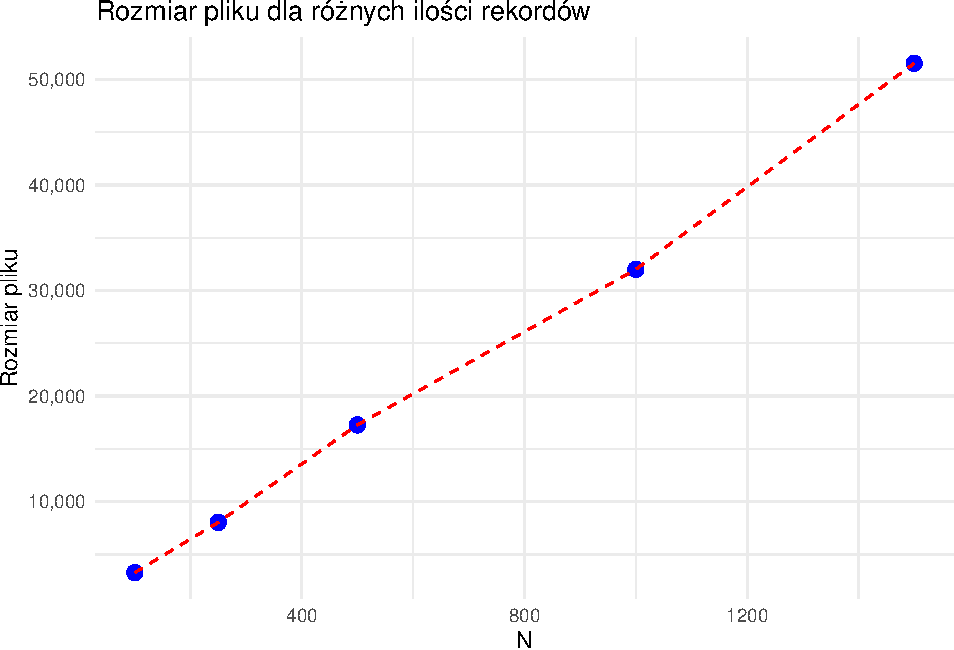
\includegraphics{sbd1_files/figure-latex/unnamed-chunk-2-1} Dla
wielkości strony 100 rekordów:

\begin{longtable}[]{@{}
  >{\centering\arraybackslash}p{(\columnwidth - 14\tabcolsep) * \real{0.1094}}
  >{\centering\arraybackslash}p{(\columnwidth - 14\tabcolsep) * \real{0.1094}}
  >{\centering\arraybackslash}p{(\columnwidth - 14\tabcolsep) * \real{0.1094}}
  >{\centering\arraybackslash}p{(\columnwidth - 14\tabcolsep) * \real{0.0938}}
  >{\centering\arraybackslash}p{(\columnwidth - 14\tabcolsep) * \real{0.1250}}
  >{\centering\arraybackslash}p{(\columnwidth - 14\tabcolsep) * \real{0.1406}}
  >{\centering\arraybackslash}p{(\columnwidth - 14\tabcolsep) * \real{0.1406}}
  >{\centering\arraybackslash}p{(\columnwidth - 14\tabcolsep) * \real{0.1719}}@{}}
\toprule\noalign{}
\begin{minipage}[b]{\linewidth}\centering
N
\end{minipage} & \begin{minipage}[b]{\linewidth}\centering
Serie
\end{minipage} & \begin{minipage}[b]{\linewidth}\centering
IO
\end{minipage} & \begin{minipage}[b]{\linewidth}\centering
Fazy
\end{minipage} & \begin{minipage}[b]{\linewidth}\centering
Zapisy
\end{minipage} & \begin{minipage}[b]{\linewidth}\centering
Odczyty
\end{minipage} & \begin{minipage}[b]{\linewidth}\centering
Teor.IO
\end{minipage} & \begin{minipage}[b]{\linewidth}\centering
Teor.Fazy
\end{minipage} \\
\midrule\noalign{}
\endhead
\bottomrule\noalign{}
\endlastfoot
10 & 5 & 12 & 3 & 6 & 6 & 12 & 3 \\
100 & 52 & 36 & 6 & 18 & 18 & 240 & 6 \\
1000 & 498 & 378 & 9 & 189 & 189 & 3600 & 9 \\
5000 & 2520 & 2424 & 12 & 1212 & 1212 & 24000 & 12 \\
10000 & 4991 & 5226 & 13 & 2613 & 2613 & 52000 & 13 \\
15000 & 7552 & 7826 & 13 & 3913 & 3913 & 78000 & 13 \\
25000 & 12489 & 14026 & 14 & 7013 & 7013 & 140000 & 14 \\
50000 & 25014 & 30030 & 15 & 15015 & 15015 & 300000 & 15 \\
\end{longtable}

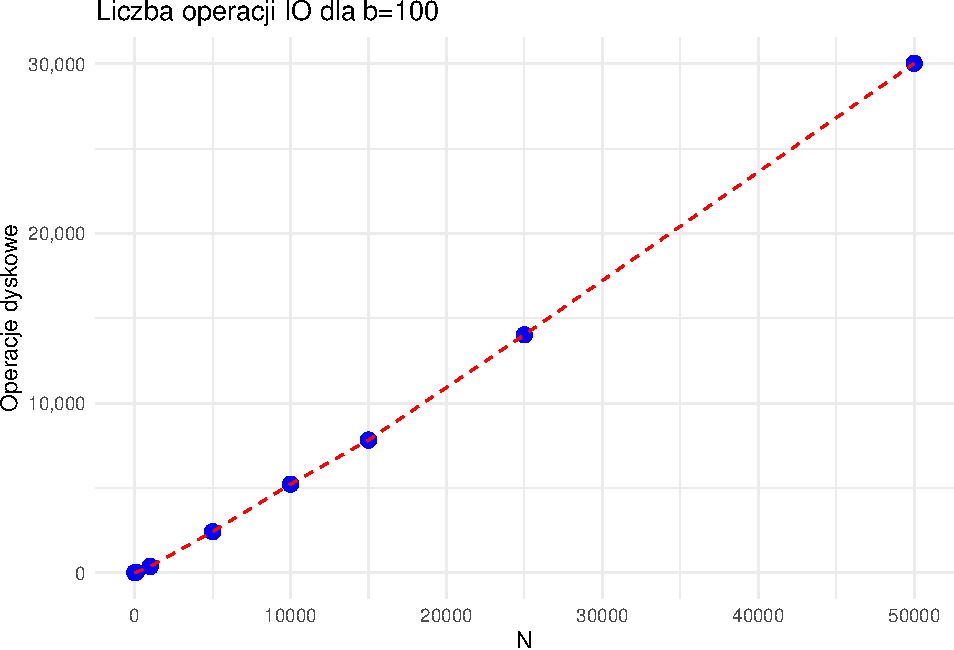
\includegraphics{sbd1_files/figure-latex/unnamed-chunk-3-1}

Jak widać, dla większej ilości strony, tym rzadziej ją wymieniamy, przez
co znacznie spadają ilości operacji dyskowych. Gdy \(N\) jest mniejsze
niż rozmiar strony, to nie ma różnicy spowodowanej rozmiarem bloków, bo
do zapisu wszystkich danych zostanie wyokrzystana tylko jedna strona na
taśmę.

\subsection{Zużycie pamięci}\label{zuux17cycie-pamiux119ci}

Zużywana pamięć w programie jest stała, jak można zaobserwować na
poniższych danych z programu \texttt{valgrind\ -\/-tool=massif}.

Dla 1000 rekordów:

\begin{figure}
\centering
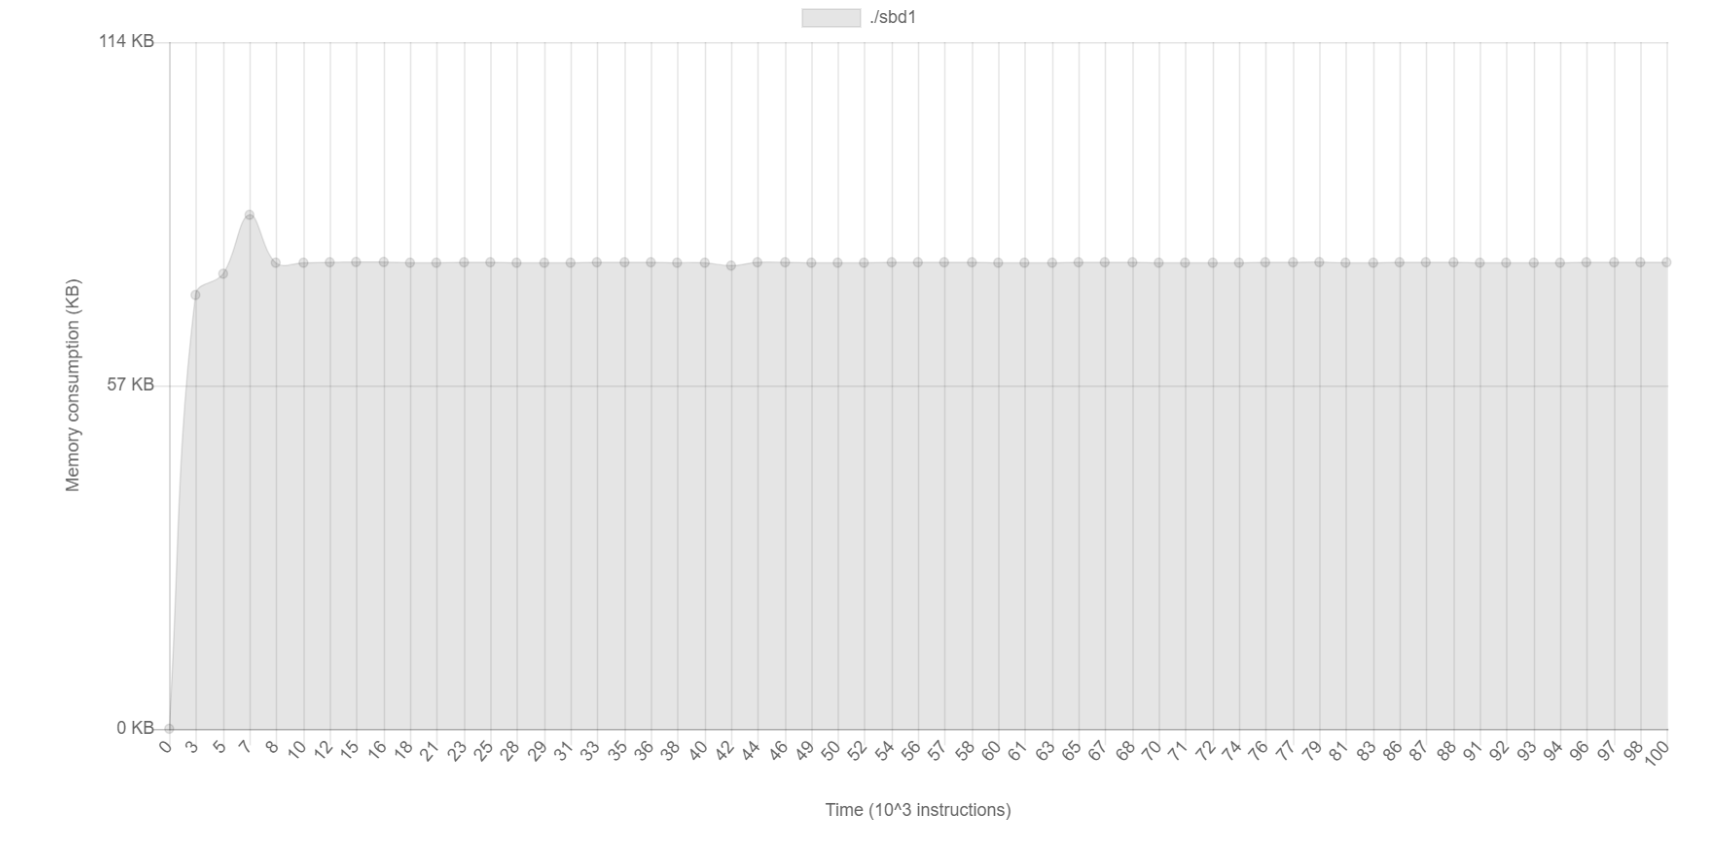
\includegraphics{../res/visualizer_small.png}
\caption{Mała ilość rekordów}
\end{figure}

Dla 5000 rekordów:

\begin{figure}
\centering
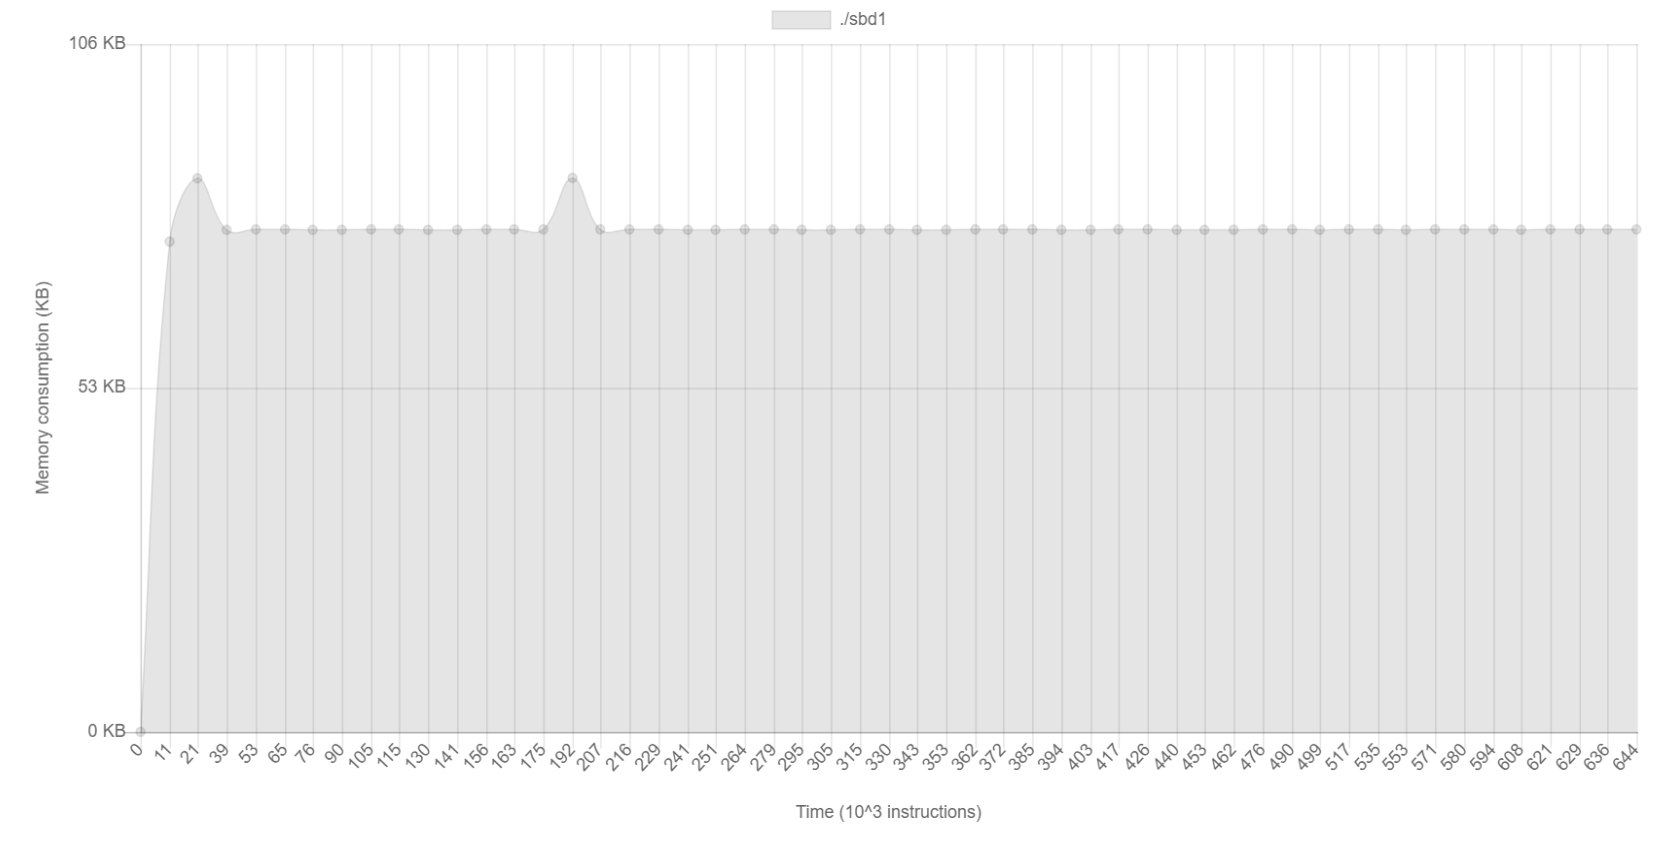
\includegraphics{../res/visualizer_medium.png}
\caption{Średnia ilość rekordów}
\end{figure}

Dla 10000 rekordów:

\begin{figure}
\centering
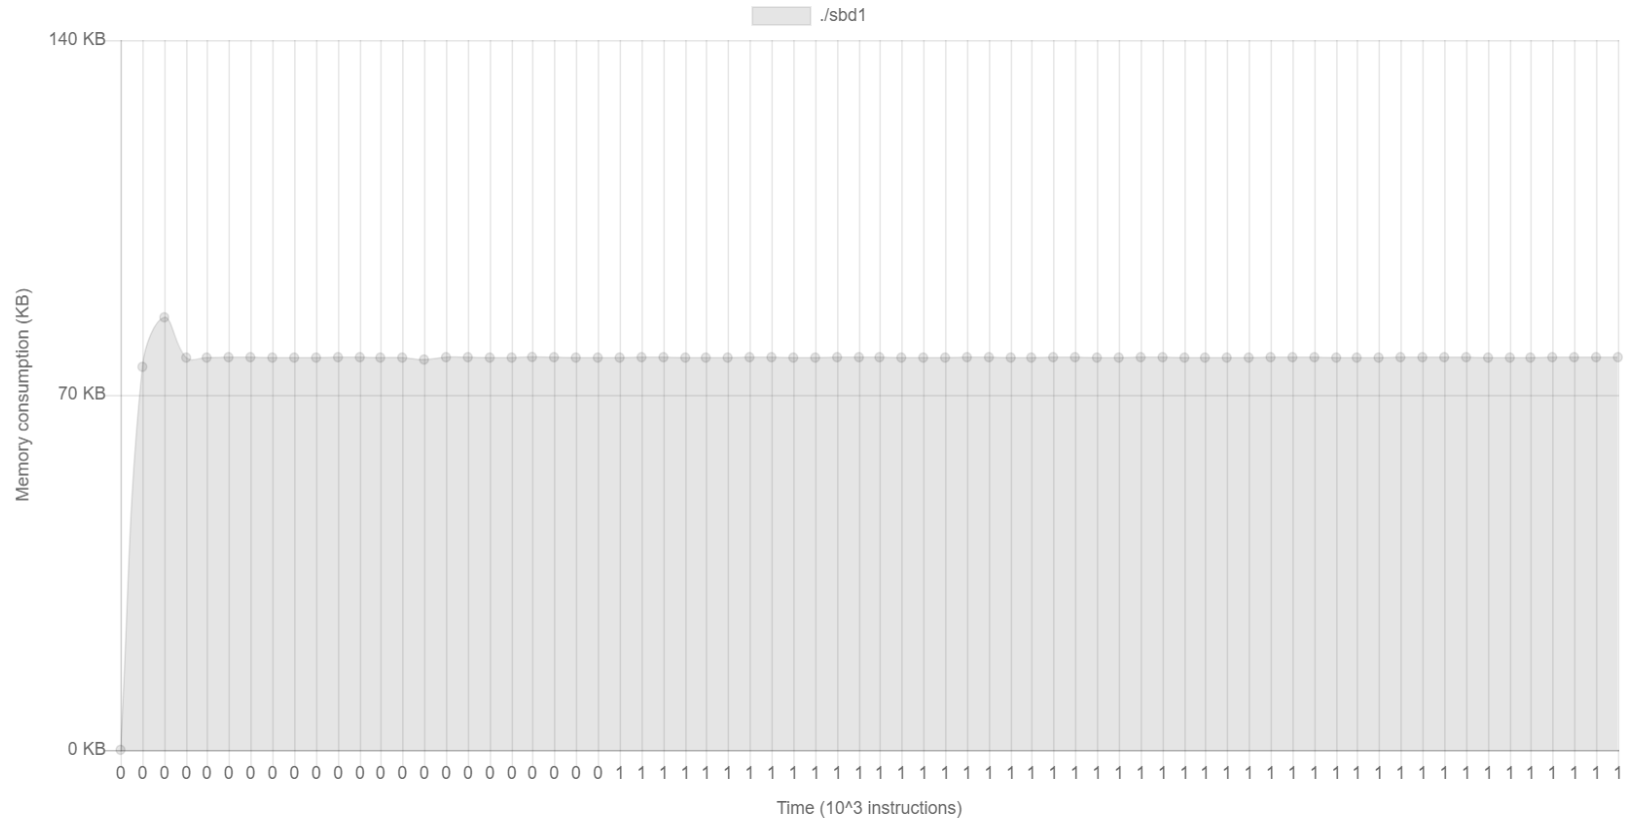
\includegraphics{../res/visualizer_big.png}
\caption{Duża ilość rekordów}
\end{figure}

Jak widać, ilość zużytej pamięci operacyjnej nie przekracza 80KB.

\section{Podsumowanie}\label{podsumowanie}

Projekt pozwolił na zrozumienie jak wielkie pliki są odczytywane z
dysku, oraz jak zaimplementować w prosty sposób własny sposób na zapis
danych tak, aby nie zużywać za dużo pamięci operacyjnej. Wyniki
eksperymentu są zgodne z oczekiwaniami rozważanymi na poziomie
teoretycznym jeśli chodzi o ilość operacji dyskowych, oraz zużycie
pamięci było stałe, więc zwiększanie liczby rekordów nie zwiększa ilości
zużywanej pamięci operacyjnej. Liczba operacji IO zwiększa się
proporcjonalnie do zwiększania współczynnika blokowania, ale
współczynnik nie ma wpływu na ilość faz algorytmu.

\end{document}
